% ===================================================================
%  Αρχείο: 15037_tikz.tex (Fragment)
%  Αυτόματη μετατροπή μέσω doc2latex.py & TikZ conversion
% ===================================================================

ΘΕΜΑ 4

Στο σχήμα φαίνονται οι γραφικές παραστάσεις των συναρτήσεις $f(x) = \sqrt{x + 3}$ και $g(x) = 3x - 1$.

\begin{center}
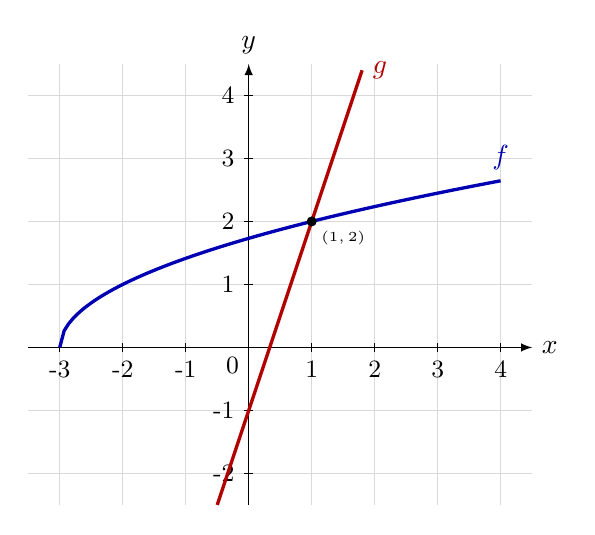
\begin{tikzpicture}[scale=0.8, >=latex]
    \draw[very thin, color=gray!30] (-3.5,-2.5) grid (4.5,4.5);
    \draw[->] (-3.5,0) -- (4.5,0) node[right] {$x$};
    \draw[->] (0,-2.5) -- (0,4.5) node[above] {$y$};
    
    \foreach \x in {-3,-2,-1,1,2,3,4}
        \draw (\x,2pt) -- (\x,-2pt) node[below, font=\small] {\x};
    \foreach \y in {-2,-1,1,2,3,4}
        \draw (2pt,\y) -- (-2pt,\y) node[left, font=\small] {\y};
    \node[below left, font=\small] at (0,0) {$0$};
    
    % f(x) = sqrt(x+3)
    \draw[very thick, color=blue!70!black, samples=100, domain=-3:4] plot (\x, {sqrt(\x+3)}) node[above] {$f$};
    
    % g(x) = 3x - 1
    \draw[very thick, color=red!70!black, samples=2, domain=-0.5:1.8] plot (\x, {3*\x - 1}) node[right] {$g$};
    
    % Intersection point (1,2)
    \filldraw (1,2) circle (2pt) node[below right, font=\tiny] {$(1,2)$};
\end{tikzpicture}
\end{center}

\begin{alist}
\item Να βρείτε το πεδίο ορισμού και τη μονοτονία των συναρτήσεων f, g.

\monades{4}

\item Να λύσετε την εξίσωση $f(x) = g(x).$

\monades{6}

\item

\begin{rlist}
\item
  Να λύσετε γραφικά την ανίσωση $f(x) < g(x).$ \monades{7}
\item
  Να επιβεβαιώσετε αλγεβρικά το αποτέλεσμα του i ερωτήματος. \monades{8}
\end{rlist}
\end{alist}
